\begin{frame}
  \frametitle{Minimisation du risque empirique}
  \begin{itemize}
  \item Principe sur lequel de nombreux algorithmes \blue{d'apprentissage
      supervisé} sont fondés.
  \item Ingrédients :
    \begin{itemize}
    \setlength{\itemsep}{5pt}
    \item \blue{Espace des hypothèses} \textcolor{gray!70}{(hypothesis space)} \\ \hspace{1em} Quels modèles peut-on apprendre ?
    \item \blue{Fonction de perte / coût / erreur} \textcolor{gray!70}{(loss / cost / error function)} \\ \hspace{1em} Comment quantifier l'erreur d'un modèle ?
    \item Algorithme d'\blue{optimisation} \\ \hspace{1em} Comment trouver un
      modèle qui fasse peu d'erreurs ?
    \end{itemize}
  \end{itemize}
\end{frame}


\begin{frame}
  \begin{center}
    \large{1. Minimisation du risque empirique}
  \end{center}
\end{frame}


\begin{frame}
  \frametitle{1.1 Espace des hypothèses}
  \begin{itemize}
  \item \blue{Données :} $\dset = \{(\xvec_1, y_1), (\xvec_2, y_2), \dots, (\xvec_n, y_n)\} $ 
    \begin{itemize}
    \item $n$ observations en $p$ dimensions : $\xvec_i \in  \RR^p$
    \item $n$ étiquettes \textcolor{gray!70}{(labels)} : $y_i \in \ycal$
    \end{itemize}
    \pause
  \item \red{Espace des hypothèses :} l'ensemble $\fcal$ des \blue{modèles} que
    l'algorithme d'apprentissage va considérer.  \pause
  \item \red{Modèles paramétriques :} on considère un ensemble paramétré de fonctions.
    \begin{itemize}
    \item[] \black{Exemple :} 
      $\fcal = \{ \xvec \mapsto {\color{MyOrange}\alpha_1} x_1^{\beta_1} +
      {\color{MyOrange}\alpha_2} x_2^{\beta_2} + \dots + {\color{MyOrange}\alpha_p} x_p^{\beta_p} \}$ \\
      Le but de l'apprentissage est de déterminer $\alpha_1, \dots, \alpha_p, \beta_1, \dots, \beta_p$ .
    \end{itemize}
  % \item \red{Modèles non-paramétriques}
  %   \begin{itemize}
  %   \item[] \black{Exemple :} $\fcal = \left\{\xvec \mapsto
  %       1 \text{ si } x_j > 1, 0 \text{ sinon.} \right\}$ \\
  %     Le but de l'apprentissage est de déterminer $j$, qui n'est pas un paramètre.    
  %   \end{itemize}
  \end{itemize}
\end{frame}

\begin{frame}
  \frametitle{1.2 Fonction de perte}
  \begin{itemize}
  \item \blue{Quantifier} l'erreur d'un modèle pour une observation.
  \item \red{Fonction de perte :} une fonction
    $L : \ycal \times \ycal \mapsto \RR$ 
  \item[] $L(y, f(\xvec))$ est d'autant plus grande que l'erreur consistant à
    prédire $f(\xvec)$ au lieu de $y$ est grande.
    \pause
    \begin{itemize}
    \item \red{Perte 0/1} \textcolor{gray!70}{(0/1 loss)} pour la classification :
      \begin{eqnarray*}
        L : & \{0, 1\} \times \{0, 1\} \rightarrow \RR \\ \nonumber
            & (y, f(\xvec)) \mapsto
              \begin{cases}
                0 & \text{ si } f(\xvec) = y \\ \nonumber
                1 & \text{ sinon.}
              \end{cases}                
      \end{eqnarray*}
      \pause
    \item \red{Perte quadratique} \textcolor{gray!70}{(quadratic loss)} pour la régression :
      \begin{eqnarray*}
        L : & \RR \times \RR \rightarrow \RR \\ \nonumber
            & (y, f(\xvec)) \mapsto (y - f(\xvec))^2
      \end{eqnarray*}      
    \end{itemize}
  \end{itemize}
\end{frame}

\begin{frame}
  \frametitle{1.3 Risque empirique}
  \begin{itemize}
  \item \red{Risque :}
    \begin{itemize}
    \item Erreur attendue du modèle sur toutes données possibles 
      \begin{mdframed}[hidealllines=true, backgroundcolor=MyLightGrey,
                       fontcolor=MyDarkGrey, leftmargin=-5pt,
                       innerleftmargin=5pt, skipabove=5pt]
      \item Formellement : l'espérance de la fonction de perte 
        \[\rcal(f) = \EE [L(Y, f(X)]\]
      \item[]
        \begin{itemize}
        \item $(\xvec_1, y_1), (\xvec_2, y_2), \dots, (\xvec_n, y_n)$
          échantillon de $(X, Y)$
        \item $X$ vecteur aléatoire réel de dimension $p$ ; $Y$ variable aléatoire
          dans $\ycal$
        \end{itemize}
      \end{mdframed}
    \end{itemize}
  \item \red{Risque empirique :} moyenne de la fonction de perte sur les
    données
    \[\rcal_{\text{emp}}(f) = \frac1n \sum_{i=1}^n L(y_i, f(\xvec_i)) \]
  \end{itemize}
\end{frame}


\begin{frame}
  \frametitle{1.4 Minimisation du risque empirique}
  \begin{itemize}
  \item \blue{Apprendre un modèle} = \blue{trouver} un modèle \blue{de l'espace des
      hypothèses} qui \blue{minimise} le \blue{risque empirique}
    \[ \hat{f} = \argmin_{f \in \fcal} \frac1n \sum_{i=1}^n L(y_i, f(\xvec_i)) \]
  \item C'est donc un problème \blue{d'optimisation}
  \item Selon l'espace des hypothèses, la fonction de perte, et la procédure
    d'optimisation choisie :
    \begin{itemize}
    \item La solution peut être unique (mais pas nécessairement)
    \item La solution peut être explicite (rarement)
    \item La solution peut être atteinte avec la précision souhaitée (parfois)
    \item La solution ne peut être déterminée que par des heuristiques 
    \end{itemize}
  \end{itemize}
\end{frame}

% \begin{frame}
%   \frametitle{1.5 Maximisation de la vraisemblance}
%   \begin{itemize}
%   \item Dans le cas d'un modèle de \blue{régression paramétrique :}
%     $\fcal = \{f_{\thetavec}  : \RR^p \rightarrow \RR ; \thetavec \in \RR^d \}$
%   \item En utilisant la \blue{perte quadratique :} $L(y, f(\xvec)) = (y - f(\xvec))^2 $
%   \item En supposant :
%     \begin{itemize}
%     \item $(\xvec_1, y_1), (\xvec_2, y_2), \dots, (\xvec_n, y_n)$ échantillon
%       de $(X, Y)$
%     \item $X$ vecteur aléatoire réel de dimension $p$ ; $Y$ variable aléatoire réelle
%     \item Il existe $f^* : \RR^p \rightarrow \RR$ telle que $Y = f^*(X) + \epsilon$
%     \item $\epsilon \sim \ncal(0, \sigma^2)$ (bruit gaussien)
%     \end{itemize}
%   \item Alors : l'estimation par maximum de vraisemblance de $\thetavec$ est
%     \blue{équivalente} à la minimisation du risque empirique
%   \end{itemize}
% \end{frame}


\begin{frame}
  \begin{center}
    \large{2. Modèles linéaires}
  \end{center}
\end{frame}

\begin{frame}
  \frametitle{2.1 Régression linéaire univariée}
  \begin{itemize}
  \item \blue{Données :} $\dset = \{(x_1, y_1), (x_2, y_2), \dots, (x_n, y_n)\} $ 
    \begin{itemize}
    \item $n$ observations dans $\RR$ : $x_i \in  \RR$ ($p=1$)
    \item $n$ étiquettes : $y_i \in \RR$
    \end{itemize}
      \begin{overprint}
        \onslide<1>\centering{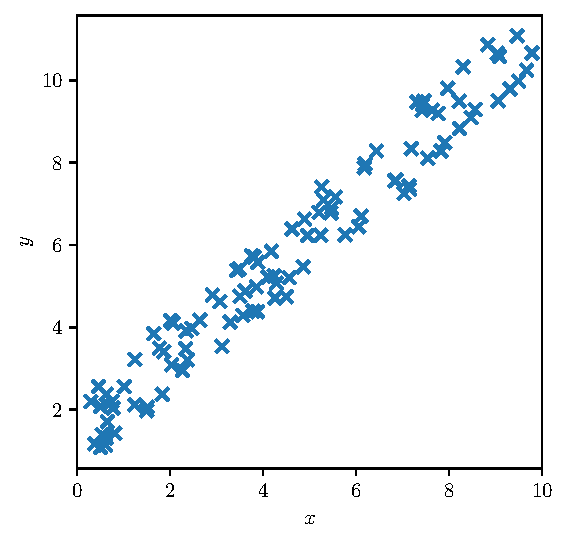
\includegraphics[width=0.5\textwidth]{figures/linreg_pb}}
        \onslide<2>\centering{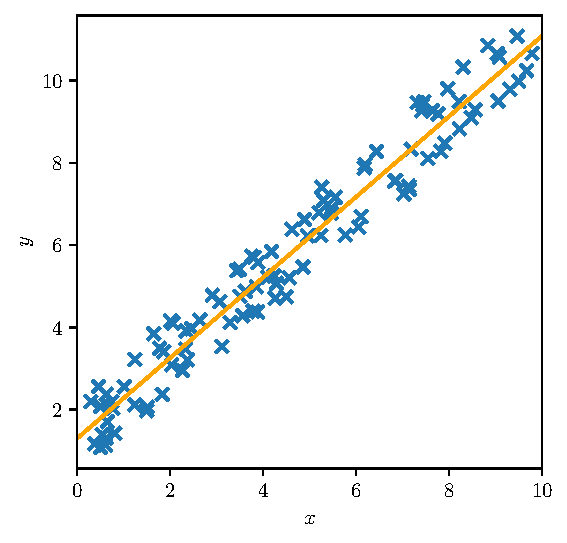
\includegraphics[width=0.5\textwidth]{figures/linreg_sol}}
      \end{overprint}
      \pause
  \item \blue{Espace des hypothèses :}  $\fcal = \{x \mapsto a x + b ; (a, b) \in \RR^2\}$ 
  \end{itemize}
\end{frame}

\begin{frame}
  \frametitle{2.1 Régression linéaire univariée}
  \begin{itemize}
  \item \blue{Espace des hypothèses :}  $\fcal = \{x \mapsto a x + b ; (a, b) \in \RR^2\}$ 
    \pause
  \item \blue{Fonction de perte :} perte quadratique $L(y, f(x)) = (y - f(x))^2$
    \pause
  \item \blue{Minimisation du risque empirique :}
    \[ (\hat{a}, \hat{b}) = \argmin_{(a,b) \in \RR^2} \frac1n \sum_{i=1}^n (y_i - (a x_i + b))^2 \]
    \pause
  \item[] \red{Méthode des moindres carrés} \textcolor{gray!70}{(ordinary least squares)} connue depuis Legendre et Gauss. 
  \end{itemize}
\end{frame}

\begin{frame}
  \frametitle{Solution}
  \begin{itemize}
  \item \blue{Par annulation des dérivées partielles :} système de deux équations à deux inconnues
  \item[] Solution explicite : 
    \begin{itemize}
    \item Si $\sum_{i=1}^n x_i^2 \neq \left(\sum_{i=1}^n x_i\right)^2,$ une \blue{unique solution}
      \[ a = \frac{\sum_{i=1}^n x_i y_i - \frac1n \sum_{i=1}^n x_i \sum_{i=1}^n y_i}{
          \sum_{i=1}^n x_i^2 - \frac1n \left(\sum_{i=1}^n x_i\right)^2}  \hspace{2em}
        b = \frac1n \sum_{i=1}^n y_i - \frac{a}{n} \sum_{i=1}^n x_i\]
      \pause
    \item Sinon, le système est \blue{indéterminé} et on a une infinité de solutions.
    \end{itemize}
  \pause
  \item \blue{Par algorithme du gradient}
  \end{itemize}
\end{frame}

\begin{frame}
  \frametitle{2.2 Régression linéaire multivariée}
  \begin{itemize}
  \item Autre nom : \blue{régression linéaire multiple}
  \item \blue{Données :} $\dset = \{(\xvec_1, y_1), (\xvec_2, y_2), \dots, (\xvec_n, y_n)\}$
    \begin{itemize}
    \item $n$ observations dans $\RR^p$ 
    \item $n$ étiquettes : $y_i \in \RR$
    \end{itemize}
  \item \blue{Espace des hypothèses :}
    \[\fcal = \left\{ \xvec \mapsto \beta_0 + \sum_{j=1}^p \beta_j x_j \, ;  \betavec \in \RR^{p+1} \right\}\]
    \pause
    \vspace{-1em}
  \item \blue{Fonction de perte :} perte quadratique $L(y, f(\xvec)) = (y - f(\xvec))^2$
    \pause
  \item \blue{Minimisation du risque empirique :}
    \[ \hat{\betavec} = \argmin_{\betavec \in \RR^{p+1}} \frac1n \sum_{i=1}^n \left(y_i - \left(\beta_0 + \sum_{j=1}^p \beta_j x_j\right)\right)^2 \]
  \end{itemize}
\end{frame}

\begin{frame}
  \frametitle{Écriture matricielle}
  \small
    \[ \hat{\betavec} = \argmin_{\betavec \in \RR^{p+1}} \frac1n \sum_{i=1}^n \left(y_i - \left(\beta_0 + \sum_{j=1}^p \beta_j x_j\right)\right)^2 \]
  \begin{itemize}
  \item La transformation 
    $\xvec \leftarrow (1, x_1, \dots, x_p)$ permet d'écrire $f(\xvec) = \langle \betavec, \xvec \rangle$ 
  \item En notant $X \in \RR^{n \times (p+1)}$ la matrice de données : $X_{i.} = \xvec_i$ et \\
    $\yvec \in \RR^n$ le vecteur des étiquettes,
    \[\sum_{i=1}^n \left(y_i - \left(\beta_0 + \sum_{j=1}^p \beta_j x_j\right)\right)^2 =
    \left(\yvec - X \betavec \right)^\top \left(\yvec - X \betavec \right)\]
\item Le problème devient 
    \[\argmin_{\betavec \in \RR^{p+1}} \frac1n 
    \left(\yvec - X \betavec \right)^\top \left(\yvec - X \betavec \right)\]
  \end{itemize}
\end{frame}


\begin{frame}
  \frametitle{Solution}
    \small
  \begin{flalign*}
    \text{Minimiser } J & : \RR^{p+1} \rightarrow \RR \\
    & \betavec \mapsto \left(\yvec - X \betavec \right)^\top
    \left(\yvec - X \betavec \right) 
  \end{flalign*}
  \begin{itemize}
  \item Problème \blue{d'optimisation convexe}
    \pause
  \item \blue{Gradient} de $J$ : $\nabla J (\betavec) = - 2 X^\top (\yvec - X \betavec)$
  \item En \blue{annulant} ce gradient, on obtient
    \[
      X^\top X \betavec = X^\top \yvec
    \]
    \vspace{-2em}
    \pause
  \item Solution :
    \begin{itemize}
    \item Si \blue{$X^\top X$ inversible}, alors $\betavec^* = \left(X^\top X\right)^{-1} X^\top \yvec$
    \item Sinon, le système est indéterminé et on a une infinité de solutions.
    \end{itemize}
  \end{itemize}
\end{frame}

\begin{frame}
  \frametitle{Inversibilité de $X^\top X$}
  \begin{itemize}
  \item $X^\top X$ est inversible ssi $X$ est de rang colonne plein.
    \pause
    \begin{itemize}
    \item Ce n'est pas le cas si $p+1 > n$ 
    \item[] i.e. s'il y a \blue{plus de variables que d'observations}
    \vspace{1em}
    \item Ce n'est pas le cas si des colonnes sont colinéaires
    \item[] i.e. si des \blue{variables sont fortement corrélées}
    \end{itemize}
    \pause
  \item L'inversion d'une matrice carrée de taille $p$ est une opération en $\mathcal{O}(p^3)$
  \item[] On utilise généralement \blue{l'algorithme du gradient} même si $X^\top X$ est inversible. 
  \end{itemize}
\end{frame}

\begin{frame}
  \frametitle{2.3 Régression logistique}
  \begin{itemize}
  \item \blue{Données :} $\dset = \{(\xvec_1, y_1), (\xvec_2, y_2), \dots, (\xvec_n, y_n)\}$
    \begin{itemize}
    \item $n$ observations dans $\RR^p$ 
    \item $n$ étiquettes : $y_i \in \{0, 1\}$ : \blue{classification binaire}
    \end{itemize}
  \pause
\item \blue{Espace des hypothèses :} Considérer des fonctions linéaires n'a pas
  de sens pour prédire une valeur binaire.  \pause
    \begin{itemize}
    \item $f$ va modéliser \blue{la probabilité d'appartenir à la classe positive}
    \pause
  \item la \red{fonction logistique} $\sigma$ transforme un réel en une ``probabilité''
    \begin{center}
    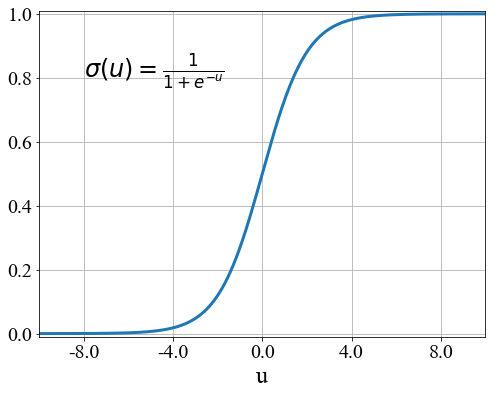
\includegraphics[width=0.38\textwidth]{figures/logistic}
  \end{center}
  \item $\fcal = \left\{\xvec \mapsto \sigma\left(\beta_0 + \langle \betavec, \xvec \rangle\right) ;  \betavec \in \RR^{p+1}\right\}$
    \end{itemize}
  \end{itemize}
\end{frame}

\begin{frame}
  \frametitle{2.3 Régression logistique}
  \begin{itemize}
  \item Fonction de perte : \red{entropie croisée} \textcolor{gray!70}{(cross-entropy)}
    \begin{flalign*}
      L :  \{0, 1\} \times ]0, 1[ & \rightarrow \RR \\ \nonumber
          (y, f(\xvec)) & \mapsto -y \log f(\xvec) - (1-y) \log (1 - f(\xvec)) % = 
        \end{flalign*}
        \begin{center}
          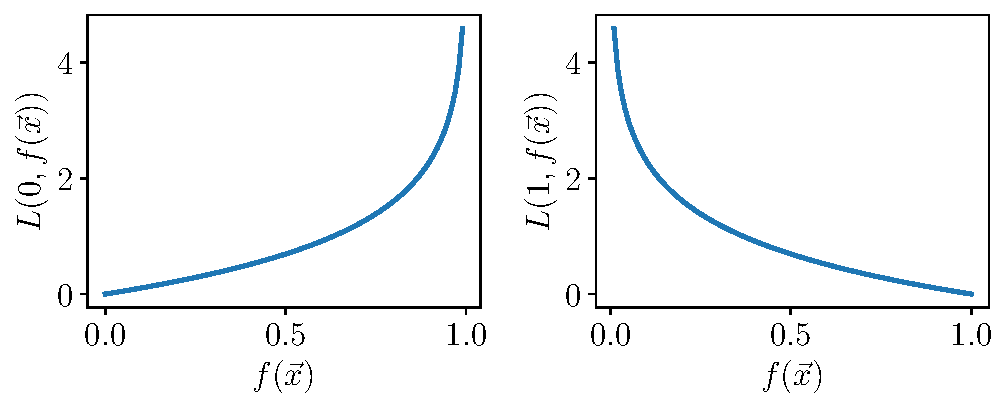
\includegraphics[width=0.8\textwidth]{figures/cross_entropy}
        \end{center}
  \end{itemize}
\end{frame}

\begin{frame}
  \frametitle{2.3 Régression logistique}
  \begin{itemize}
  \item Fonction de perte : \red{entropie croisée} \textcolor{gray!70}{(cross-entropy)}
    \begin{flalign*}
      L :  \{0, 1\} \times ]0, 1[ & \rightarrow \RR \\ \nonumber
          (y, f(\xvec)) & \mapsto -y \log f(\xvec) - (1-y) \log (1 - f(\xvec)) % = 
        \end{flalign*}
  \item[] Si $y=1$, alors $L = -\log f(\xvec)$. La perte va donc être minimisée si $f(\xvec)\rightarrow1$. 
  \item[] Si $y=0$, alors $L = -\log(1-f(\xvec))$. La perte va donc être minimisée si $f(\xvec)\rightarrow0$. 
  \end{itemize}
\end{frame}

\begin{frame}
  \frametitle{2.3 Régression logistique}
  \begin{itemize}
  \item \blue{Espace des hypothèses :}
    $\fcal = \{\xvec \mapsto \sigma\left(\beta_0 + \langle \betavec, \xvec
      \rangle\right) ; \betavec \in \RR^{p+1}\}$
  \item \blue{Fonction de perte :}
    $L : (y, f(\xvec))  \mapsto -y \log f(\xvec) - (1-y) \log (1 - f(\xvec))$
  \item \blue{Minimisation du risque empirique :}
    \footnotesize
    \[\argmin_{\betavec \in \RR^{p+1}} \frac1n \sum_{i=1}^n
      -y_i \log \sigma\left(\beta_0 + \langle \betavec, \xvec_i \rangle\right)
      - (1-y_i) \log \left(1 - \sigma\left(\beta_0 + \langle \betavec, \xvec_i \rangle\right)\right)
    \]
  \end{itemize}
\end{frame}

\begin{frame}
  \frametitle{2.3 Régression logistique - Solution}
  \begin{itemize}
  \item \blue{Minimiser}
    {\footnotesize \[J : \betavec \mapsto \sum_{i=1}^n -y_i \log \sigma\left(\beta_0 + \langle
      \betavec, \xvec_i \rangle\right) - (1-y_i) \log \left(1 -
      \sigma\left(\beta_0 + \langle \betavec, \xvec_i \rangle\right)\right)\]}
  \pause
  \item $J$ est une fonction \blue{convexe} de $\betavec$
  \pause
  \item En utilisant $\sigma^\prime (u) = \sigma(u) (1-\sigma(u)),$
    \[
      \nabla J(\betavec) = \sum_{i=1}^n \left( y_i - \frac1{1 + \exp - \left(\beta_0 +
            \langle \betavec, \xvec_i \rangle \right)} \right)
    \]
  \item[$\Rightarrow$] Pas de solution explicite.
    \pause
  \item On utilise donc systématiquement \blue{l'algorithme du gradient.}
  \end{itemize}
\end{frame}

\begin{frame}
  \frametitle{2.3 Régression logistique - Interprétation}
  \begin{itemize}
  \item Le \blue{coefficient de régression}
    $\beta_j$ peut être interprété comme la contribution de la variable correspondante ($x_j$) au modèle
  \item À condition que les variables soient \blue{centrées-réduites} pour être à la même échelle :
    \[
      x_j \leftarrow \frac{x_j - \overline{x_j}}{\sigma_j}
    \]
    \begin{itemize}
    \item $\overline{x_j}$ : moyenne de $x_j$ sur les données
    \item $\sigma_j$ : écart-type de $x_j$ sur les données
    \end{itemize}
  \item Attention à calculer $\overline{x_j}$ et $\sigma_j$ sur le jeu
    d'entraînement uniquement, pour ne pas toucher au jeu de test.
  \end{itemize}
\end{frame}

\begin{frame}
  \frametitle{2.3 Régression logistique - Entropie croisée et maximisation de vraisemblance}
  \begin{itemize}
    \item On écrit $P(y_i\,|\,\xvec_i; \theta)$ la probabilité de prédire la classe $y_i$ (donc de prédire la classe correcte). 
  \item Probabilité que toutes les prédictions sont bonnes est la probabilité jointe de $N$ bonnes prédictions :  
  \begin{equation*}
    \prod_{i=1}^NP(y_i | \xvec_i; \theta)
  \end{equation*}
  \end{itemize}
\end{frame}

\begin{frame}
  \frametitle{2.3 Régression logistique - Entropie croisée et maximisation de vraisemblance}
  \begin{itemize}
    \item Approche de maximisation de la vraisemblance : 
    \begin{eqnarray*}
    \theta^{\ast} &=& \argmax_{\theta} \prod_{i=1}^NP(y_i | \xvec_i; \theta) \\
                  &=& \argmax _{\theta} \sum_{i=1}^N\log P(y_i | \xvec_i; \theta)\\
                  &=& \argmin_{\theta} - \sum_{i=1}^N\log P(y_i | \xvec_i; \theta)
    \end{eqnarray*}    
  \end{itemize}
\end{frame}

\begin{frame}
  \frametitle{2.3 Régression logistique - Entropie croisée et maximisation de vraisemblance}
  \begin{itemize}
    \item Si on suppose qu'on prédit la probabilité a posteriori, on peut écrire : 
    \begin{equation*}
    \log P(y_i|(\xvec_i; \theta) = y_i \log (f(\xvec_i; \theta)) + (1-y_i)\log (1-f(\xvec_i; \theta))
    \end{equation*}
    et on obtient : 
    \begin{equation*}
    \theta^{\ast} = \argmin_{\theta} - \sum_{i=1}^N [y_i \log (f(\xvec_i; \theta)) + (1-y_i)\log (1-f(\xvec_i; \theta))]
    \end{equation*}
    \item Nous voyons que minimiser l'entropie croisée est équivalent à maximiser la vraisemblance.
  \end{itemize}
\end{frame}



% -------------------------------------------------
% Linear Discriminant Analysisd
\begin{frame}
\frametitle{2.4 Analyse discriminante linéaire - règle Bayesienne 1/4}
%\begin{block}{Probabilité conditionnelle et probabilité jointe}
  \begin{itemize}
  \item Soient $X$ et $Y$ deux variables aléatoires, $P(X)$ et $P(Y)$ leurs probabilités marginales, $P(X,Y)$ la probabilité jointe et $P(X\,|\,Y)$ la \red{probabilité conditionnelle} de $X$ sous condition de $Y$.
    \begin{itemize}
    \item La \red{probabilité jointe} peut s'écrire alors:
    \begin{equation}
      P(X,Y) = P(X\,|\,Y)P(Y)
    \end{equation}
    \item et la \red{probabilité marginale} est la somme des probabilités jointes pour toutes les valeurs de $Y$:
    \begin{equation}
      P(X) = \sum_Y P(X,Y) = \sum(P(X|Y)P(Y)
    \end{equation}
  \end{itemize}
  \end{itemize}
%\end{block}
\end{frame}

\begin{frame}
\frametitle{2.4 Analyse discriminante linéaire - règle Bayesienne 2/4}
\begin{itemize}
\item Comme $P(X,Y)=P(Y,X)$ on obtient directement le théorème Bayésien:
\begin{equation}
  P(Y \, | \, X) = \frac{P(X \, | \, Y)P(Y)}{P(X)}
\end{equation}
\item Ici $X$ et $Y$ sont des variables discrètes, mais une règle presque identique peut être définie pour des variables continues. Pour cela il faut remplacer les probabilités par des densités de probabilité. 
\end{itemize}

% Here, we assume that $Y$ is a discrete variable (classes) and $X$ is a continuous variable (measurements). We thus obtain: 
% \begin{equation}
%   P(Y \, | \, X) = \frac{p(X \, | \, Y)P(Y)}{p(X)}
% \end{equation}

\end{frame}

\begin{frame}{2.4 Analyse discriminante linéaire - règle Bayesienne 3/4}

\begin{itemize}
%\begin{block}{Règle Bayesienne de classification}
  \item \red{Probabilité postérieure}: Soit $\xvec \in \mathbb{R}^P$ avec une densité de probabilité $p(\xvec)$ et $y \in \{1 \ldots, K\}$ une variable discrète. La probabilité a posteriori $P(y=k\,|\,\xvec)$ est donc :
  \begin{equation}
    P(y=k \, | \, \xvec) = \frac{p(\xvec \, | \, y=k) P(y=k)}{p(\xvec)}
  \end{equation}
  \item \red{La règle Bayesienne de classification}: \emph{Choisis la classe qui maximise} $P(y=k|\xvec)$:
  \begin{equation}
    \hat{y}(\xvec) = \arg\max_k P(y=k \, | \, \xvec) = \arg\max_k p(\xvec\,|\,y=k)P(y=k)
  \end{equation}
%\end{block}
\end{itemize}
\end{frame}


\begin{frame}{2.4 Analyse discriminante linéaire - règle Bayesienne 4/4}

\begin{itemize}
  \item La règle Bayesienne de classification simplement dit que la meilleure classe à choisir est celle avec la plus grande probabilité étant donné l'observation. 
  \item Cette probabilité peut être estimée à partir de la distribution des observations pour la classe et de la probabilité \emph{a priori}. 
  \item Cette règle est importante parce qu'elle donne le meilleur classifieur possible, si l'on connaît les distributions des observations $p(\xvec\,|\,y=k)$ et les probabilités \emph{a priori} $P(y=k)$.
  \item Malheureusement, ce n'est pas le cas. Ces distributions doivent être estimées à partir des données d'apprentissage. 
\end{itemize}

\end{frame}

\begin{frame}{2.4 Analyse discriminante linéaire - cas binaire}

\begin{itemize}
\item On assume que l'on essaie de résoudre un problème binaire, cad $y \in \{1, 2\}$. La règle Bayésienne dit alors qu'il faut choisir la classe 1 si : 

\begin{equation*}
\frac{p(\xvec|y=1)P(y=1)}{p(\xvec|y=2)P(y=2)} > 1
\end{equation*}

\item On peut appliquer le $log$ aux deux côté de cette équation. On obtient donc l'expression suivante : 

\begin{equation}\label{equ:lda:condition}
\log{ \frac{p(\xvec|y=1)P(y=1)}{p(\xvec|y=2)P(y=2)} } > 0
\end{equation}
\end{itemize}
\end{frame}

\begin{frame}{2.4 Analyse discriminante linéaire - Supposition de normalité}
\begin{figure}[htb]
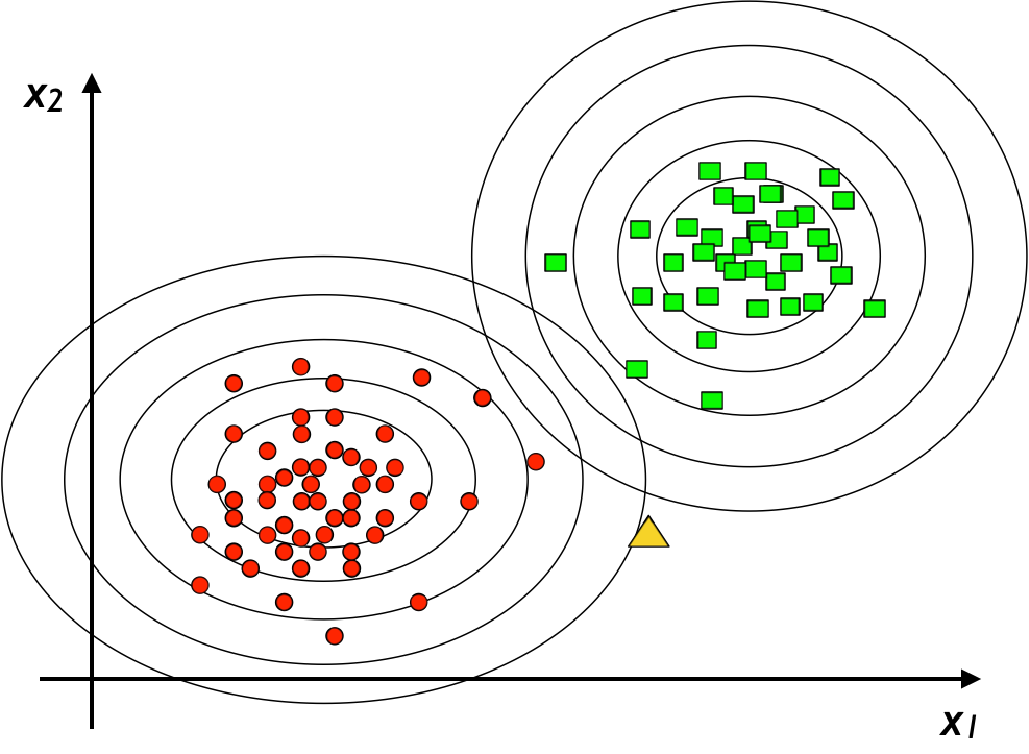
\includegraphics[width=0.5\textwidth]{figures/LDA.pdf}
\end{figure}
\begin{itemize}
\item On suppose que les descripteurs sont distribués normalement pour chacune des classes : 
\begin{equation}\label{equ:lda:normal}
p(\xvec|y=k)=\frac{1}{(2\pi)^{\frac{p}{2}}|\Sigma_k|^{\frac{1}{2}}}e^{-\frac{1}{2}(\xvec-\mu_k)^T\Sigma_k^{-1}(\xvec-\mu_k)}
\end{equation}
\end{itemize}
\end{frame}

\begin{frame}{2.4 Analyse discriminante linéaire}
\frametitle{Analyse discriminante linéaire}
\begin{itemize}
\item Avec les expressions (\ref{equ:lda:normal}) et (\ref{equ:lda:condition}) et l'hypothèse supplémentaire que les matrices de covariance sont identiques pour toutes les classes, cad
$\Sigma_1 = \Sigma_2 = \Sigma$, on obtien l'analyse discrimnante linéaire {\bf Linear Discriminant Analysis, LDA}:
\begin{equation*}
K + \xvec^T\Sigma^{-1}(\mu_1-\mu_2) - \frac{1}{2}(\mu_1-\mu_2)^T\Sigma^{-1}(\mu_1+\mu_2) > 0
\end{equation*}
avec $K=\log{\frac{P(y=1)}{P(y=2)}} + \frac{1}{2}\log{\frac{|\Sigma_2|}{|\Sigma_1|}}$
\item On observe : 
\begin{itemize}
  \item Il s'agit d'un classifier linéarie. 
  \item L'expression implique l'inversion d'une matrice de covariance (instable pour des descripteurs corrélés). 
  %\item $LDA$ is an old technique, but it is still used in practice. 
\end{itemize} 
\end{itemize} 
\end{frame}




% \begin{frame}
%   \frametitle{Régressions polynomiales}
% \end{frame}

%%% Local Variables:
%%% mode: latex
%%% TeX-master: "2022-01-azencott"
%%% End:
